\documentclass{article}
\usepackage[utf8]{inputenc}
\usepackage{tikz}
\usepackage{geometry}
\usepackage{amsmath}
\usepackage{float}
\usepackage{txfonts}
\usepackage{amssymb}
\usepackage{mathtools}
\usepackage[colorlinks]{hyperref}
\usepackage{float}

% http://tex.stackexchange.com/a/43009/20959
\DeclarePairedDelimiter\abs{\lvert}{\rvert}%
\DeclarePairedDelimiter\norm{\lVert}{\rVert}%

% http://tex.stackexchange.com/questions/5223/command-for-argmin-or-argmax#comment28205_5255
\DeclareMathOperator*{\argmin}{\arg\!\min}


\usetikzlibrary{bayesnet,calc,patterns,angles,quotes,decorations.pathreplacing,bending,intersections}

\newcommand\independent{\protect\mathpalette{\protect\independenT}{\perp}}
\def\independenT#1#2{\mathrel{\rlap{$#1#2$}\mkern2mu{#1#2}}}
\newcommand\given{\;\vert\;}

\title{Scribe Notes}
\author{Saul Shanabrook and Abe Handler}
\date{6 October 2016}

\begin{document}

\maketitle

\tableofcontents


\section{Least Means Squares}
We have some pairs of data:

$$
\{(\boldsymbol{x_i}, y_i) \given i=1\ldots n\}
$$

And we want to model $y$ as some function of $x$:

$$
y_i = \boldsymbol{\theta}^{\top} \boldsymbol{x_i} + \epsilon_i
$$

We will approach how to find $\boldsymbol{\theta}$ from a linear algebra perspective, then move to a probabilistic one. 


\subsection{Linear Algebra Constraint Satisfaction}
Let $x^j_i$ be the $j$th dimension of the $i$th $x$ observation. Where:

$$
\boldsymbol{x_i} = \begin{bmatrix}
x^1_i \\
x^2_i \\
\vdots \\
x^K_i
\end{bmatrix}
$$


For illustration purposes we will consider a 2D space, where $K=2$. We will visualize some values on the space of the two $X$ dimensions.

\begin{align*}
\boldsymbol{x_i} & \in \varmathbb{R}^2 \\
y_i & \in \varmathbb{R} \\
\epsilon_i & \in \varmathbb{R} \\
\boldsymbol{\theta} & \in \varmathbb{R}^2 \\
\end{align*}


\begin{figure}[h!]
\centering
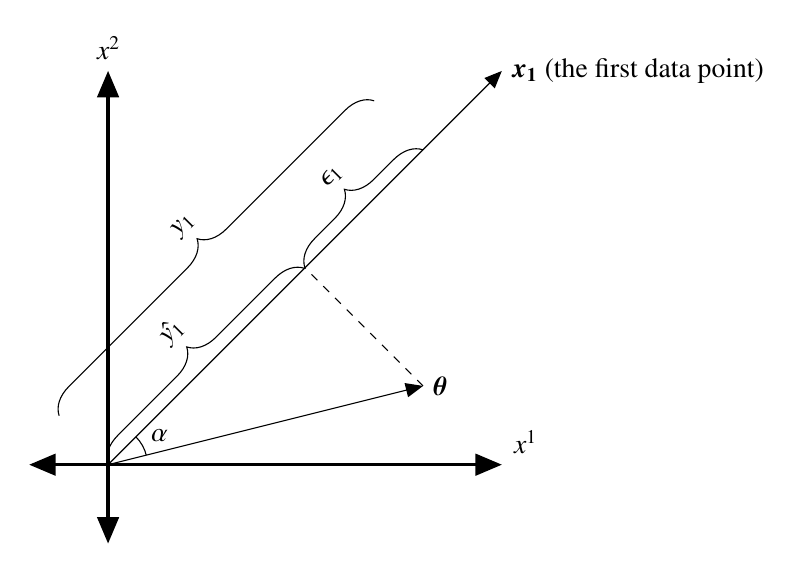
\begin{tikzpicture}
    
    % axis
    \coordinate (orig) at (0,0);
    \draw[<->, very thick]
        (-1,0) --
        (5,0) node[above right] {$x^1$};
        
    \draw[<->, very thick]
        (0,-1) --
        (0,5) node[above] {$x^2$};
    
    
    % x_1
    \coordinate (x_1) at (5,5);
    \draw[->]
        (0, 0) --
        (x_1) node[right] {$\boldsymbol{x_1}$ (the first data point)};
    
    % theta
    \coordinate (theta) at (4,1);
    \draw[->]
        (0, 0) --
        (theta) node[right] {$\boldsymbol{\theta}$};
    
    
    % y hat
    \pic [draw, -, "$\alpha$", angle eccentricity=1.5] {angle = theta--orig--x_1};
    
    \coordinate (y_hat) at ($(orig)!(theta)!(x_1)$);
    
    \draw [-, dashed]
        (theta) --
        (y_hat);
    
    \draw [
            decorate,
            decoration={
                brace,
                amplitude=10pt,
                raise=0pt
            }
        ]
        (orig) --
        (y_hat)
        node [midway,above=10pt, sloped] {$\hat{y_1}$};
    
    % y
    \coordinate (y) at ($0.8*(x_1)$);
    
    \draw [
            decorate,
            decoration={
                brace,
                amplitude=10pt,
                raise=25pt
            }
        ]
        (orig) --
        (y)
        node [midway,above=35pt, sloped] {$y_1$};
    
    % error
    \draw [
            decorate,
            decoration={
                brace,
                amplitude=10pt
            }
        ]
        (y_hat) --
        (y)
        node [midway,above=10pt, sloped] {$\epsilon_1$};

\end{tikzpicture}
\end{figure}

The estimated value of $y$, $\hat{y}$, is the magnitude
$\boldsymbol{\theta}$ projected onto $\boldsymbol{x_1}$.

\begin{align*}
\hat{y_1} & \triangleq \norm*{\boldsymbol{\theta}} \cos \alpha \\
    & \triangleq \boldsymbol{\theta}^{\top} \frac{ \boldsymbol{x_1}}{\norm*{\boldsymbol{x_1}}} \\
\end{align*}

$\epsilon_1$ is the difference between the estimated and actual value of $y$.

$$
\epsilon_1 = y_1 - \hat{y_1}
$$


To fit $\boldsymbol{\theta}$ to this data point, we want to set it so that $\epsilon_i$ is 0, so that:

$$
    y_1 = \boldsymbol{\theta}^{\top} \frac{ \boldsymbol{x_1}}{\norm*{\boldsymbol{x_1}}}
$$

Now we just have a constraint satisfaction problem.

If we add another data point:


\begin{figure}[H]
\centering
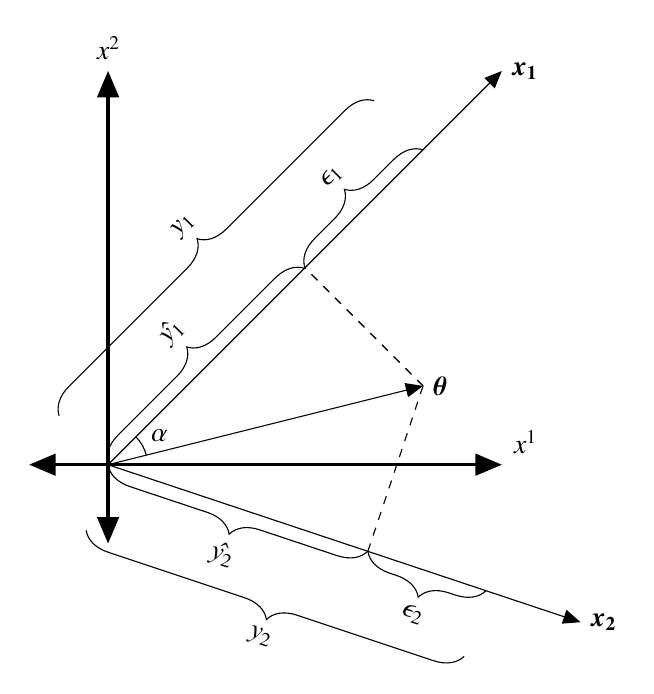
\begin{tikzpicture}
    
    % axis
    \coordinate (orig) at (0,0);
    \draw[<->, very thick]
        (-1,0) --
        (5,0) node[above right] {$x^1$};
        
    \draw[<->, very thick]
        (0,-1) --
        (0,5) node[above] {$x^2$};
    
    
    % x_1
    \coordinate (x_1) at (5,5);
    \draw[->]
        (0, 0) --
        (x_1) node[right] {$\boldsymbol{x_1}$};
    
    % theta
    \coordinate (theta) at (4,1);
    \draw[->]
        (0, 0) --
        (theta) node[right] {$\boldsymbol{\theta}$};
    
    
    % y hat
    \pic [draw, -, "$\alpha$", angle eccentricity=1.5] {angle = theta--orig--x_1};
    
    \coordinate (y_hat) at ($(orig)!(theta)!(x_1)$);
    
    \draw [-, dashed]
        (theta) --
        (y_hat);
    
    \draw [
            decorate,
            decoration={
                brace,
                amplitude=10pt,
                raise=0pt
            }
        ]
        (orig) --
        (y_hat)
        node [midway,above=10pt, sloped] {$\hat{y_1}$};
    
    % y
    \coordinate (y) at ($0.8*(x_1)$);
    
    \draw [
            decorate,
            decoration={
                brace,
                amplitude=10pt,
                raise=25pt
            }
        ]
        (orig) --
        (y)
        node [midway,above=35pt, sloped] {$y_1$};
    
    % error
    \draw [
            decorate,
            decoration={
                brace,
                amplitude=10pt
            }
        ]
        (y_hat) --
        (y)
        node [midway,above=10pt, sloped] {$\epsilon_1$};
    
    
    % x_2
    \coordinate (x_2) at (6,-2);
    \draw[->]
        (0, 0) --
        (x_2) node[right] {$\boldsymbol{x_2}$};
    
    % y_2 hat
    
    \coordinate (y_2_hat) at ($(orig)!(theta)!(x_2)$);
    
    \draw [-, dashed]
        (theta) --
        (y_2_hat);
    
    \draw [
            decorate,
            decoration={
                mirror,
                brace,
                amplitude=10pt
            }
        ]
        (orig) --
        (y_2_hat)
        node [midway,below=10pt, sloped] {$\hat{y_2}$};
    
    % y
    \coordinate (y_2) at ($0.8*(x_2)$);
    
    \draw [
            decorate,
            decoration={
                mirror,
                brace,
                amplitude=10pt,
                raise=25pt
            }
        ]
        (orig) --
        (y_2)
        node [midway,below=35pt, sloped] {$y_2$};
    
    % error
    \draw [
            decorate,
            decoration={
                mirror,
                brace,
                amplitude=10pt
            }
        ]
        (y_2_hat) --
        (y_2)
        node [midway,below=10pt, sloped] {$\epsilon_2$};

\draw [-, dashed]
    (theta) --
    (y_hat);

\end{tikzpicture}
\end{figure}

We have another constraint on $\boldsymbol{\theta}$:

$$
y_2 = \boldsymbol{\theta}^{\top} \frac{ \boldsymbol{x_2}}{\norm*{\boldsymbol{x_2}}}
$$

We can reorganize this pair of equations as:

% how can we do this?

\begin{align*}
\begin{bmatrix}
y_1 \\[0.5em]
y_2 \\[0.5em]
\end{bmatrix} & = 
\begin{bmatrix}
\boldsymbol{x_1}^{\top} \\[0.5em]
\boldsymbol{x_2}^{\top} \\[0.5em]
\end{bmatrix}
\boldsymbol{\theta} \\
\boldsymbol{Y} & = \boldsymbol{X} \boldsymbol{\theta}  \\
\end{align*}

If we solve this for $\boldsymbol{\theta}$, we get the \hypertarget{normal}{\textbf{normal equations}}:

$$
\left(\boldsymbol{X}^{\top}\boldsymbol{X}\right)^{-1}\boldsymbol{X}^{\top}\boldsymbol{Y} = \boldsymbol{\theta}
$$

We can solve these in one shot, for all the data, to get an optimal $\boldsymbol{\theta}$. So far, we have only looked at this when the number of data points is equal to the dimensions of $X$, i.e. when $n=K$.

\subsubsection{Iterative Calculation}
Instead of calculating this in one shot with all the data, what if we want to calculate it iteratively with bits of the data at a time?

Let's say we start with some initialization of the parameters, $\boldsymbol{\theta^{\left(0\right)}}$. Then when we encounter the first data point, $\left(\boldsymbol{x_1}, y_1\right)$, we should move our parameters to $\boldsymbol{\theta^{\left(1\right)}}$ so that they fit this data point.

\begin{figure}[h!]
\centering
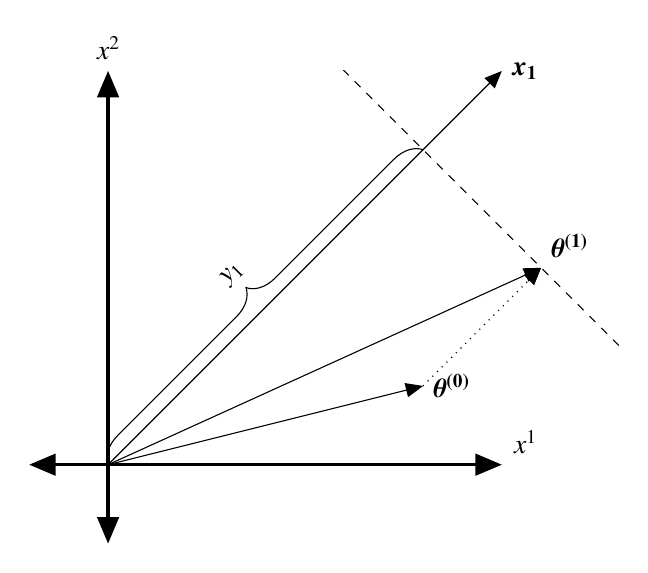
\begin{tikzpicture}
    
    
    % axis
    \coordinate (orig) at (0,0);
    \draw[<->, very thick]
        (-1,0) --
        (5,0) node[above right] {$x^1$};
        
    \draw[<->, very thick]
        (0,-1) --
        (0,5) node[above] {$x^2$};
    
    
    % x_1
    \coordinate (x_1) at (5,5);
    \draw[->]
        (0, 0) --
        (x_1) node[right] {$\boldsymbol{x_1}$};
    

    % theta
    \coordinate (theta) at (4,1);
    \draw[->]
        (0, 0) --
        (theta) node[right] {$\boldsymbol{\theta^{\left(0\right)}}$};
    
    
    % y hat

    \coordinate (y_hat) at ($(orig)!(theta)!(x_1)$);
    

    

    % y
    \coordinate (y) at ($0.8*(x_1)$);
    
    \draw [
            decorate,
            decoration={
                brace,
                amplitude=10pt
            }
        ]
        (orig) --
        (y)
        node [midway,above=10pt, sloped] {$y_1$};

    \clip (-1,-1) rectangle (6.5, 5);

    \coordinate (y_1_left) at ($(y)!4!90:(x_1)$);
    \coordinate (y_1_right) at ($(y)!4!-90:(x_1)$);
    \draw[dashed] (y_1_left) -- (y_1_right);

    \coordinate (theta_1) at ($(y_1_left)!(theta)!(y_1_right)$);
    \draw[->, dotted] (theta) -- (theta_1)
        node[above right] {$\boldsymbol{\theta^{\left(1\right)}}$};
    \draw[->] (orig) -- (theta_1);

    
\end{tikzpicture}
\end{figure}

As you can see, we can update $\boldsymbol{\theta}$ by moving it in the direction of of $\boldsymbol{x_1}$ by the difference of actual value of $y_1$ and the current projected value.

$$
 \boldsymbol{\theta^{(1)}} = \boldsymbol{\theta^{(0)}} + \left( y_1 -  \boldsymbol{\theta^{(0)}}^{\top} \frac{ \boldsymbol{x_1}}{\norm*{\boldsymbol{x_1}}} \right) \frac{ \boldsymbol{x_1}}{\norm*{\boldsymbol{x_1}}}
$$

Now the projection of $\boldsymbol{\theta^{(1)}}$ onto $\boldsymbol{x_1}$ gives $y_1$.


If we add another constraint, $\left(\boldsymbol{x_2}, y_2\right)$, we should should update $\boldsymbol{\theta}$ again with this constraint.

The general form for updating $\boldsymbol{\theta}$ is:


\begin{align*}
 \boldsymbol{\theta^{(t+1)}} = & \boldsymbol{\theta^{(t)}} + \left( y_i -  \boldsymbol{\theta^{(t)}}^{\top} \frac{ \boldsymbol{x_i}}{\norm*{\boldsymbol{x_i}}} \right) \frac{ \boldsymbol{x_i}}{\norm*{\boldsymbol{x_i}}} \\
  = & \boldsymbol{\theta^{(t)}} + \rho \left( y_i -  \boldsymbol{\theta^{(t)}}^{\top} \boldsymbol{x_i} \right) \boldsymbol{x_i} \\
\end{align*}

Where $i$ is the index of the data pair we are currently updating  $\boldsymbol{\theta}$ with and $\rho=\frac{1}{\norm*{\boldsymbol{x_i}}^2}$. \href{https://en.wikipedia.org/wiki/Stochastic_approximation#Robbins.E2.80.93Monro_algorithm}{Robbins and Monro proved} that we can adjust $\rho$ to speed up or slow down fitting $\boldsymbol{\theta}$, to the data. We want to set $\rho$ high at the beginning and decrease it as $\boldsymbol{\theta}$ approaches the optimal that fits the data. As long as $0<\rho<\frac{2}{\norm*{\boldsymbol{x_i}}^2}$, it is guaranteed to converge to the right answer. Both the order of the data and the schedule of $\rho$ can have large impacts on the performance of this algorithm. So far, this only works when the number of equations is equal to the number of unknowns.

\subsection{Calculus Based}

We are often interested in situations where $n >> k$, however. In those cases we cannot fit $\boldsymbol{\theta}$ exactly. Instead, we pick one, $\boldsymbol{\hat{\theta}}$,  that tries to minimize the $\epsilon$:

\begin{align*}
    \epsilon_i & = \text{the amount I violate the $i$th constraint} \\
    & = y_i - \hat{y_i} \\
    & = y_i - \boldsymbol{\theta}^{\top} \boldsymbol{x_i} \\
    \\
    \boldsymbol{\hat{\theta}} &= \argmin_{\boldsymbol{\theta}} \sum^N_{i=1} \epsilon_i^2
\end{align*}

If we solve this using calculus, we get the \hyperlink{normal}{normal equations}.



\subsection{Geometric Linear Algebra}
Finally we will look at LMS from a geometric perspective, as taught by \href{http://www.stat.berkeley.edu/~freedman/}{David Freedman}. Let $\boldsymbol{\hat{Y}}$ be the projection of $\boldsymbol{\theta}$ onto the columns of $\boldsymbol{X}$:

\begin{align*}
    \boldsymbol{\hat{Y}} & = \boldsymbol{X} \boldsymbol{\theta} \\
    \\
    \boldsymbol{Y} & \in \varmathbb{R}^N \\
    \boldsymbol{X} & \in \varmathbb{R}^{N \times K} \\
    \boldsymbol{\theta} & \in \varmathbb{R}^K \\
    \\ 
    \boldsymbol{X} & =  \begin{bmatrix}
\boldsymbol{x_1}^{\top} \\[0.5em]
\vdots \\[0.5em]
\boldsymbol{x_N}^{\top} \\[0.5em]
\end{bmatrix} \\
    \boldsymbol{\hat{Y}}  = \boldsymbol{X} \boldsymbol{\theta} & = \begin{bmatrix}
    \\
    \boldsymbol{x^1}\\
    \\
    \end{bmatrix} \theta^1 + \hdots + \begin{bmatrix}
    \\
    \boldsymbol{x^K}\\
    \\
    \end{bmatrix} \theta^K \\
\end{align*}

Here $\boldsymbol{Y}$ is outside of the column space of $\boldsymbol{X}$. If we project $\boldsymbol{Y}$ onto the column space of $\boldsymbol{X}$, we get $\boldsymbol{\hat{Y}}$:


\begin{figure}[H]
\centering
\begin{tikzpicture}[rotate around x=-80]
    

    % axis
    \coordinate (orig) at (0,0,0);

    \draw[->, very thick]
        (orig) --
        (3,0, 0) node[above right] {$\boldsymbol{x^1}$};
        
    \draw[->, very thick]
        (orig) --
        (0,3,0) node[above] {$\boldsymbol{x^2}$};
    
        \draw[->, very thick]
        (orig) --
        (2,2,5) node[above] {$\boldsymbol{Y}$};
    
        \draw[-] (-2, -2, 0) -- (-2, 5, 0) -- (5, 5, 0) node[above] {column space of $\boldsymbol{X}$} -- (5, -2, 0) -- (-2, -2, 0);
        
        \draw[-, dotted] (2,2,5) -- (2, 2, 0);
    
    \draw[->] (orig) -- (2, 2, 0) node[right] {$\boldsymbol{\hat{Y}}$};

    
\end{tikzpicture}
\end{figure}



$$
\boldsymbol{\hat{Y}} = \left( \boldsymbol{X}^{\top} \boldsymbol{X} \right)^{-1} \boldsymbol{X}^{\top} \boldsymbol{Y}
$$

The error vector (the dotted line in the diagram) is orthogonal to the column space of $\boldsymbol{X}$. So:

\begin{align*}
    \boldsymbol{X}^{\top} \left(\boldsymbol{Y} - \boldsymbol{\hat{Y}}\right) & = 0 \\
    \boldsymbol{X}^{\top} \left(\boldsymbol{Y} - \boldsymbol{X} \boldsymbol{\theta}\right) & = 0 \\
    \boldsymbol{X}^{\top} \boldsymbol{Y} -\boldsymbol{X}^{\top}  \boldsymbol{X} \boldsymbol{\theta} & = 0 \\
    \left(\boldsymbol{X}^{\top}\boldsymbol{X}\right)^{-1}\boldsymbol{X}^{\top}\boldsymbol{Y} & = \boldsymbol{\theta}\\
\end{align*}

So we get the normal equations again.

\clearpage

\section{Exponential Families}

Now we have a set of tools to tackle regression. As a refresher we define this as learning some $\boldsymbol{\theta}$ to minimize the error, $\epsilon$, when pairs of $\left(\boldsymbol{X}, y\right)$ data are known: 


\begin{figure}[H]
\centering
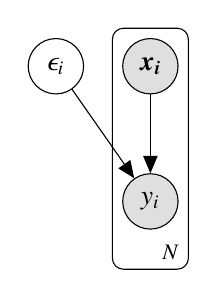
\begin{tikzpicture}

  \node[obs] (x) {$\boldsymbol{x_i}$};
  \node[obs, below=of x] (y) {$y_i$};
  \node[latent, above=of y, xshift=-1.2cm]  (e) {$\epsilon_i$};

  % Connect the nodes
  \edge {x,e} {y} ; %

  % Plates
  \plate {yx} {(x)(y)} {$N$} ;


\end{tikzpicture}
\end{figure}

\begin{align*}
    y_i & = \boldsymbol{x_i}^{\top} \boldsymbol{\theta} + \epsilon_i \\
    \epsilon_i & \sim \mathcal{N}\left(0, \sigma^2 \right)
\end{align*}

In many cases we are interested in values of $y_i$ that are only a subset of all real numbers. For example, it could be a number of coin flips, ${0, 1}$, or the number of votes in an election, $[0, \infty)$. Probability gives us one set of tools to deal with both discrete and continuous cases.We will use measure theory to understand these different valid ranges of $y_i$.

With measure theory, we might say we have a box and we want to determine it's size. It tells us that  we can use $a = w \times l$, where $w$ and $l$ and positive. In probability, we want to measure the size of events in the sample space, which is constrained in certain ways:

\begin{itemize}
    \item No measures are greater than 1
    \item Size of the whole space is 1
    \item Measuring none of the space gives us 0
\end{itemize}

This means that a point in space has probability 0, which is why with continuous random variables we talk about probability \textit{density}. We define the probability the probability of an event as $\int r(dx)$, where $r(dx)$ is just to account for discrete distributions as well.

We define the exponential family as:

$$
\Pr(x \mid \boldsymbol {\eta }) = \underbrace{h(x)}_{\mathclap{\text{normalization}}} \exp ( \underbrace{{\boldsymbol {\eta }}^{\top}}_{\text{canonical param.}} \overbrace{\boldsymbol{T}(x)}^{\mathclap{\text{sufficient statistic}}} - \underbrace{A(\boldsymbol {\eta })}_{\mathclap{\text{cumulative generating fn.}}} )
$$

\end{document}
